\chapter{Results and discussion}

\section{Final dataset composition}

\begin{figure}[ht]
    \centering
    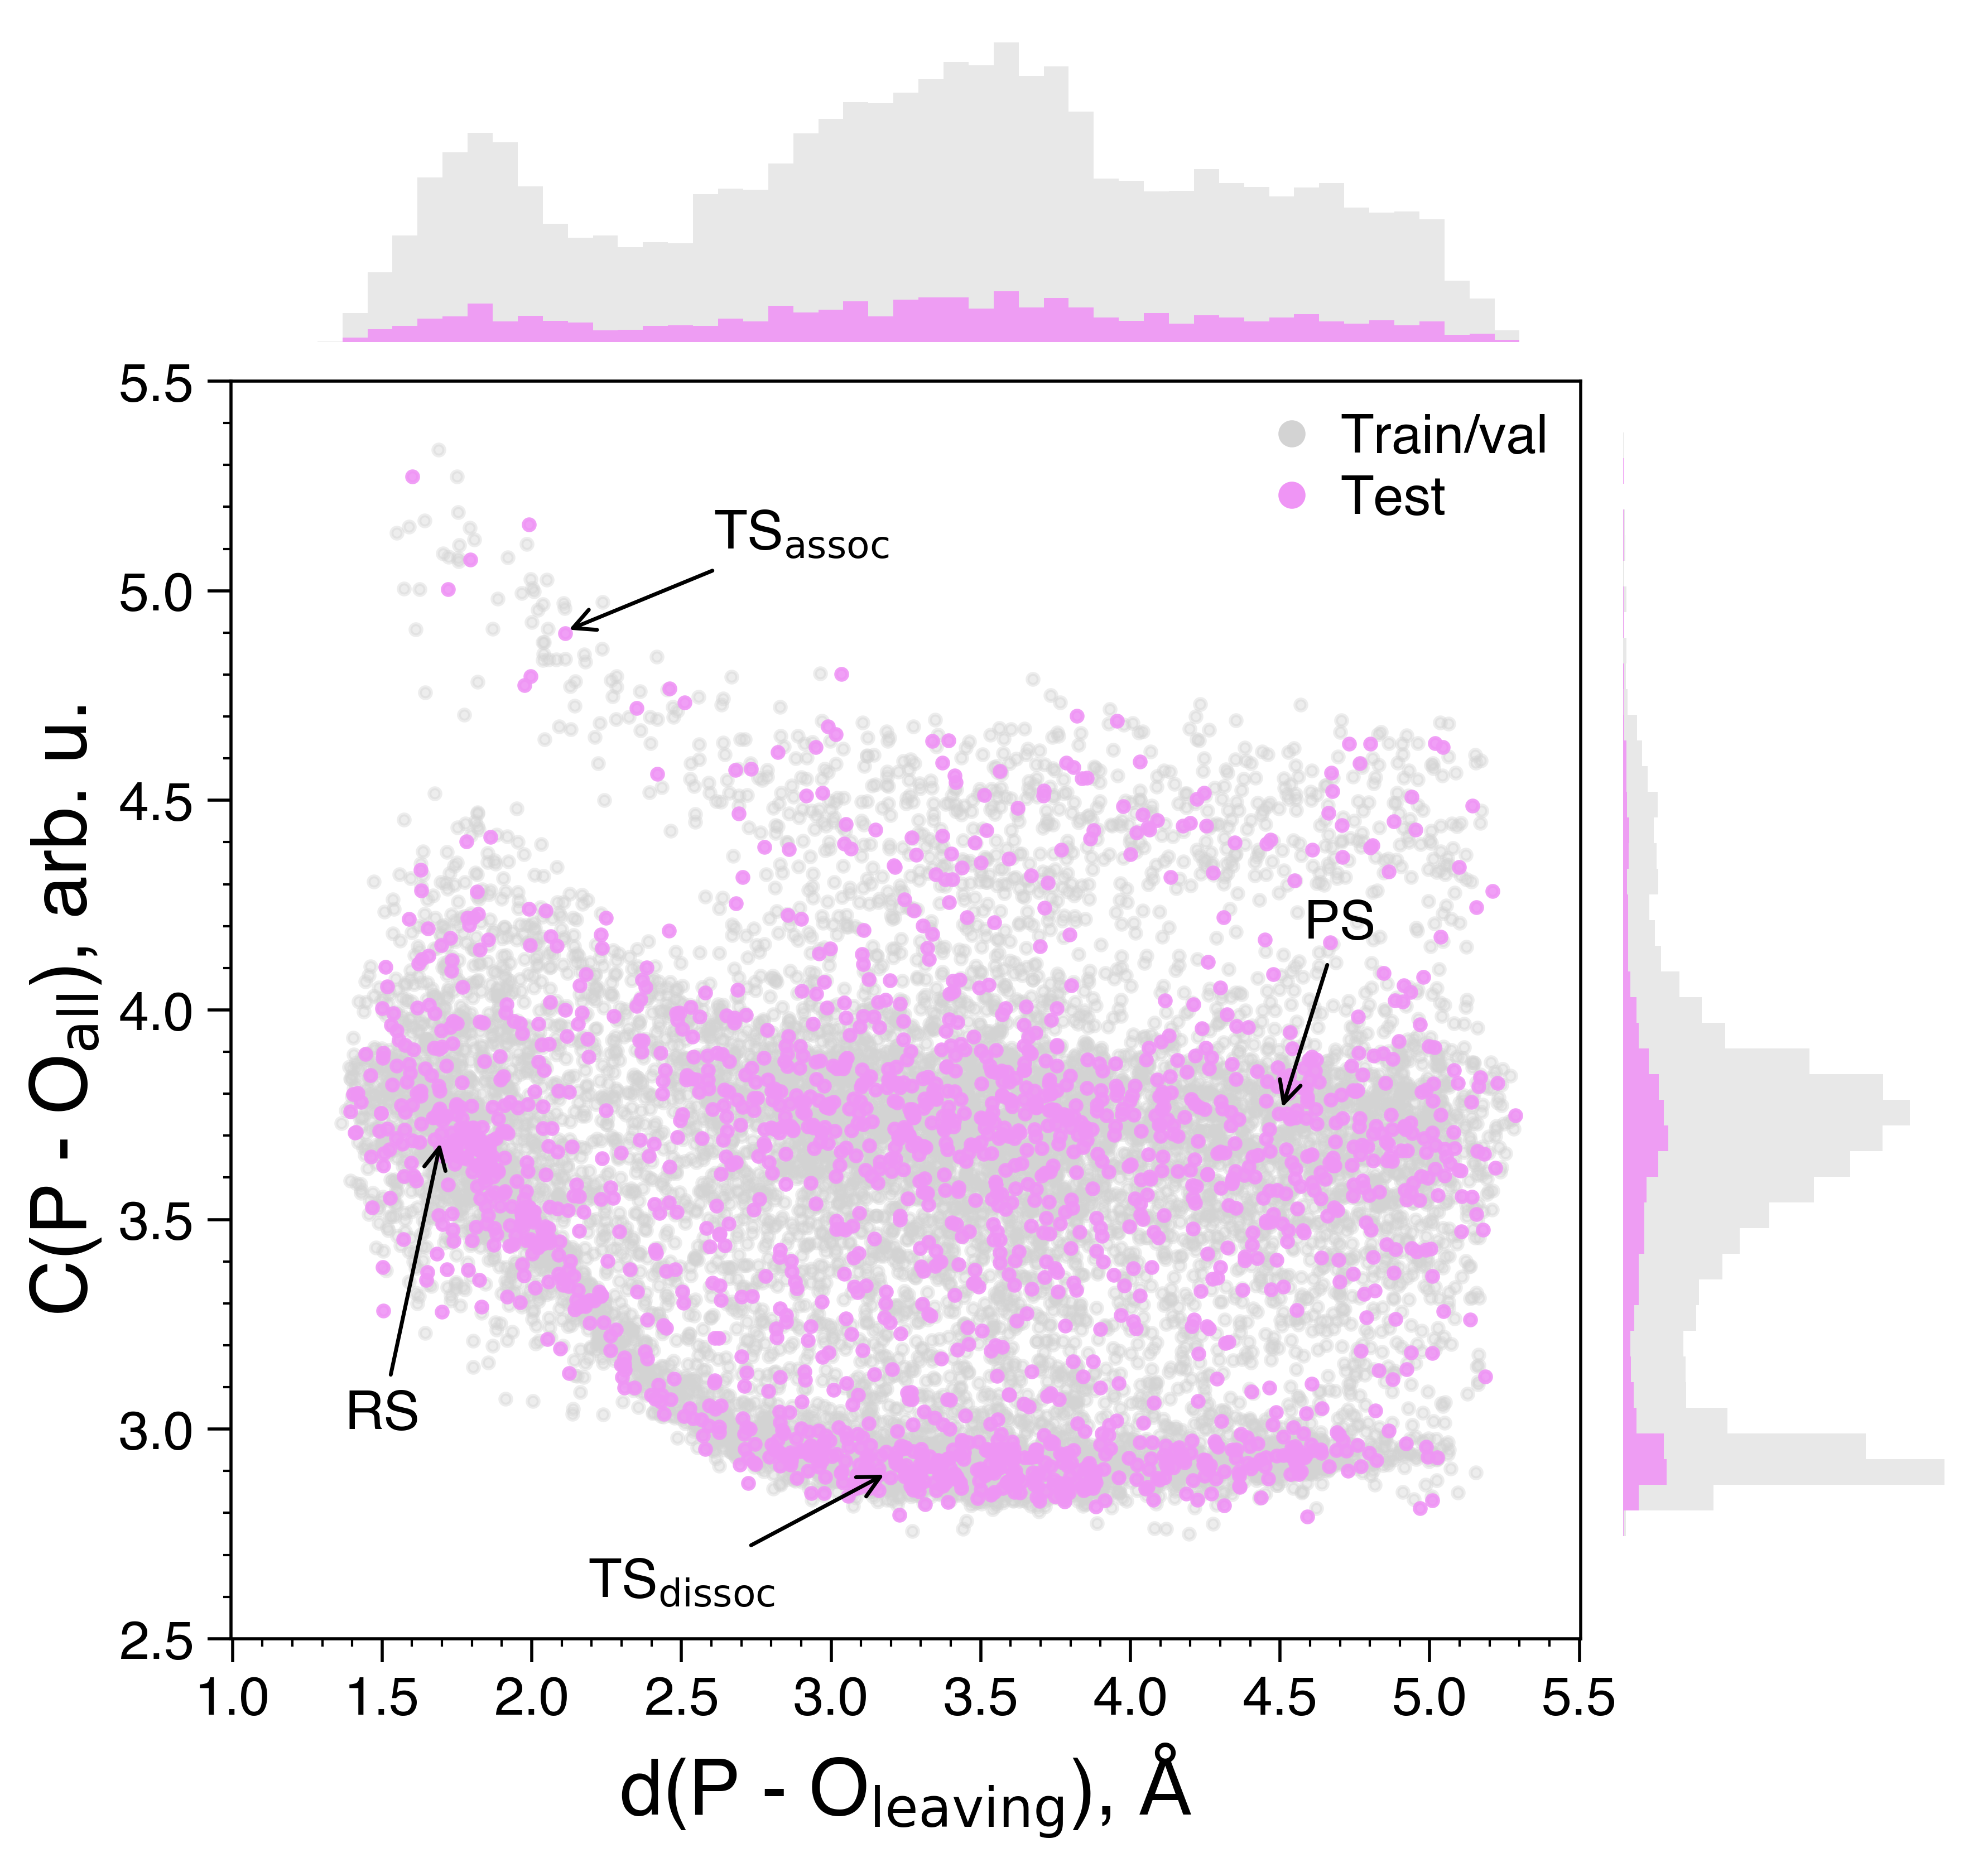
\includegraphics[width=0.6\textwidth]{Figures/4_Results/results_final_dataset_with_histograms.png}
    \caption{Final dataset composition projected on the two CVs space. In total, 12,000 data points are visualised for the training and validation parts, as well as 1,800 points for the test set. RS stands for the reactants state, PS for the product state, and TS for the transition state. 50 bins were used to produce the histograms.}
    \label{fig:final_dataset}
\end{figure}


%%%%%%%%%%%%%%%%%%%%%%%%%%%%%%%%%%%%%%%%%%%%%%%%%%%%%%%%%%%%%%%%%%%%%%%%%%%%%%%%
\clearpage
\section{Accuracy and performance of the neural network potential}

\begin{figure}[ht]
    \centering
    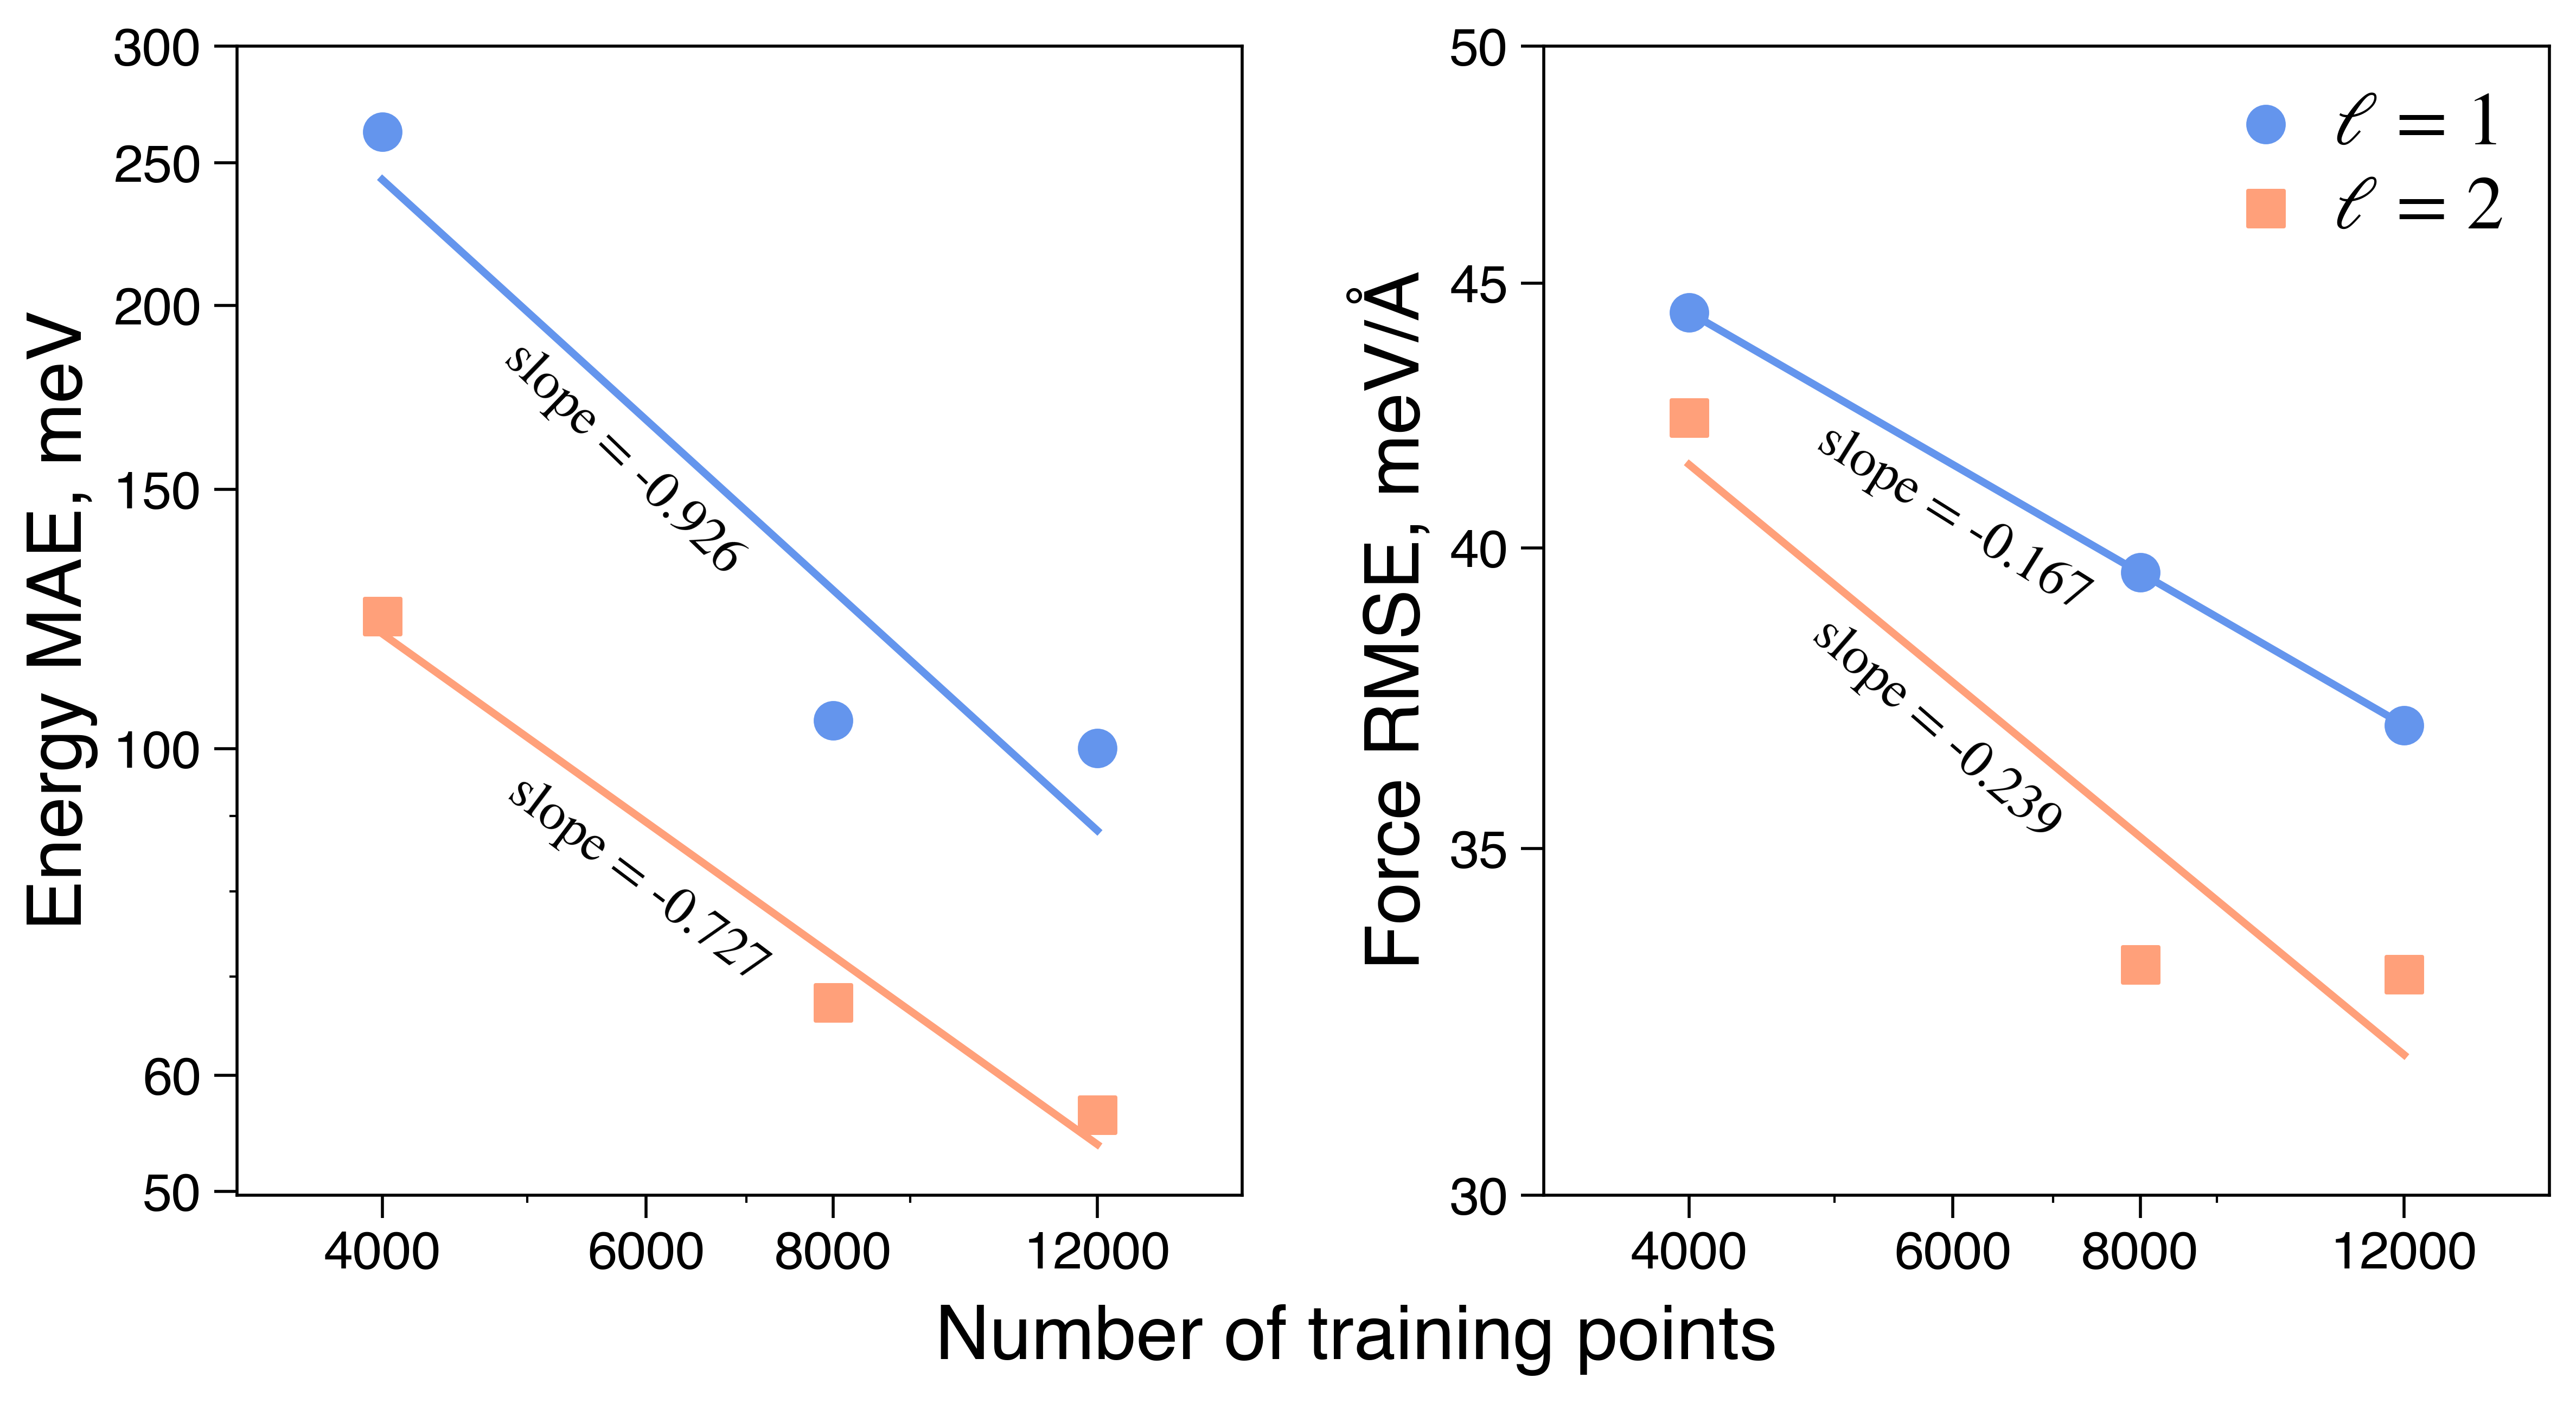
\includegraphics[width=0.8\textwidth]{Figures/4_Results/results_nnp_loglog_energy_force.png}
    \caption{Log-log plot of the errors in the energy and forces for the neural network potential with the respect to the training dataset size. In all cases, the errors were calculated on the final test set of 1,200 data points.}
    \label{fig:nnp_log-log}
\end{figure}

\begin{figure}[ht]
    \centering
    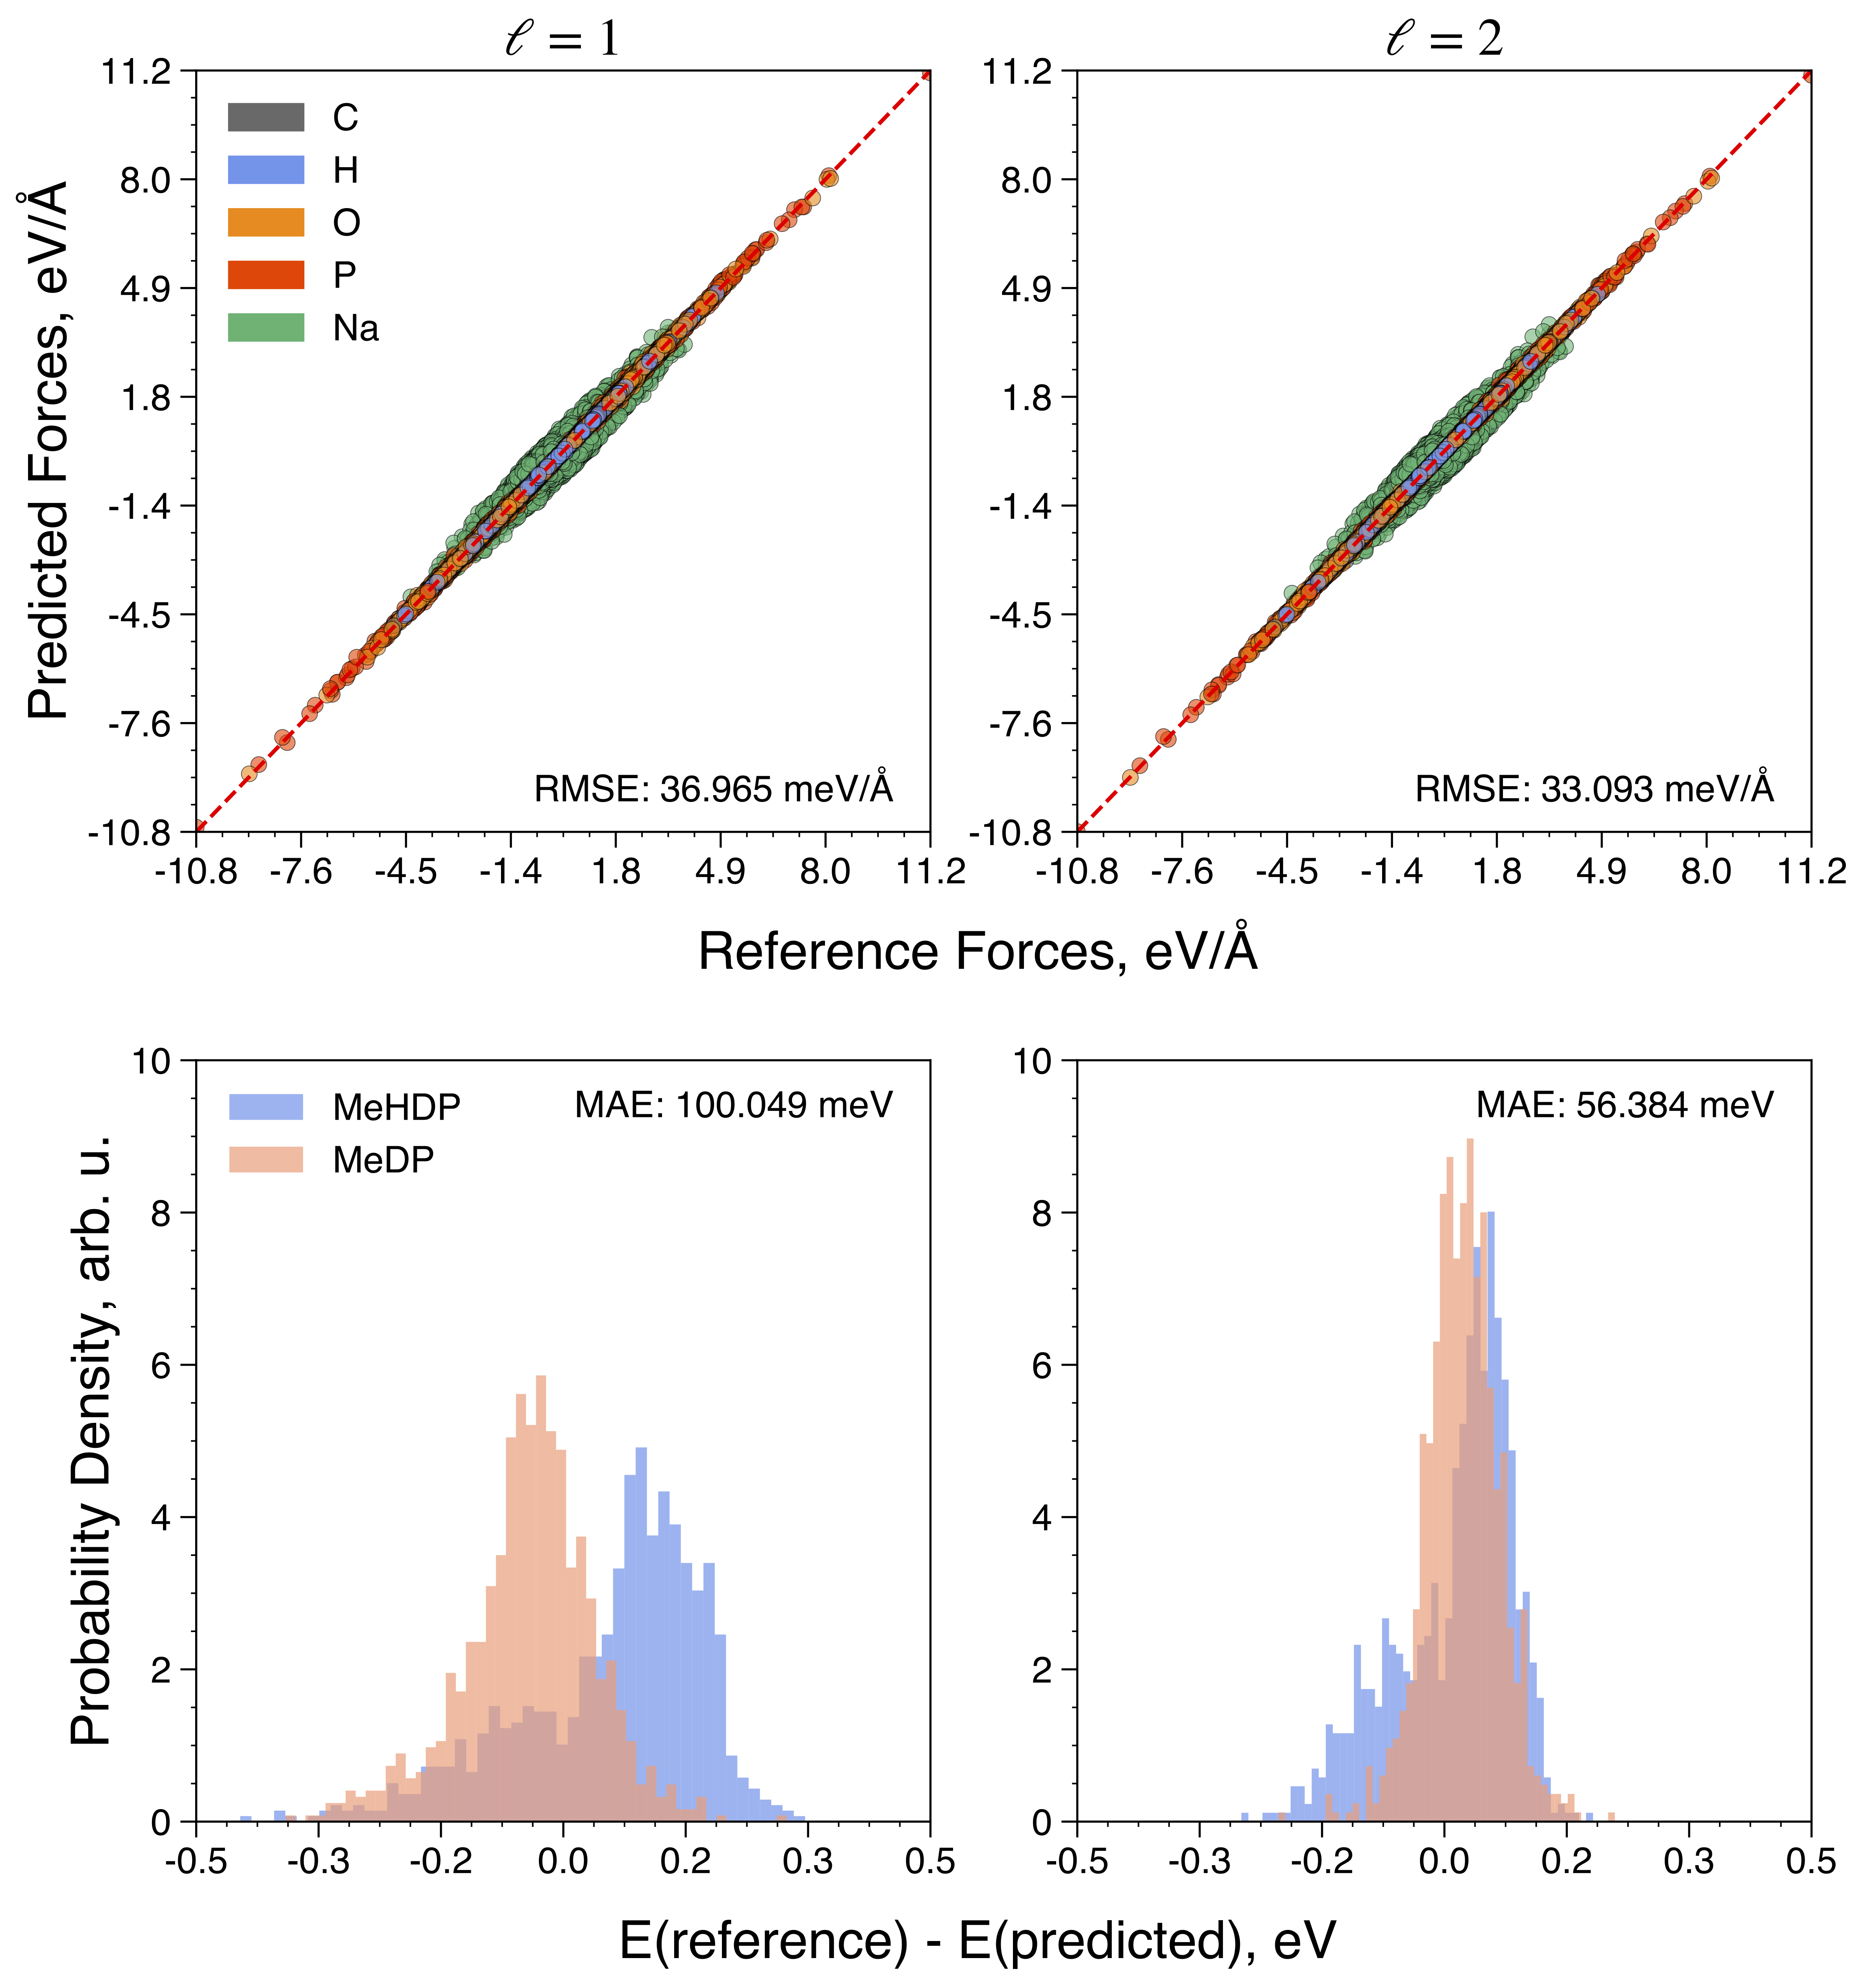
\includegraphics[width=0.8\textwidth]{Figures/4_Results/results_nnp_accuracy_l-1_l-2.png}
    \caption{Accuracy of the neural network potential trained on 12,000 data points. The left panel shows the errors in the forces and energy for the tensor rank $\ell=1$ and the right panel shows the errors for $\ell=2$. The errors are calculated as the difference between the neural network potential and the reference DFT values. For the histograms, the number of bins was set to 50.}
    \label{fig:nnp_accuracy}
\end{figure}

\begin{figure}[ht]
    \centering
    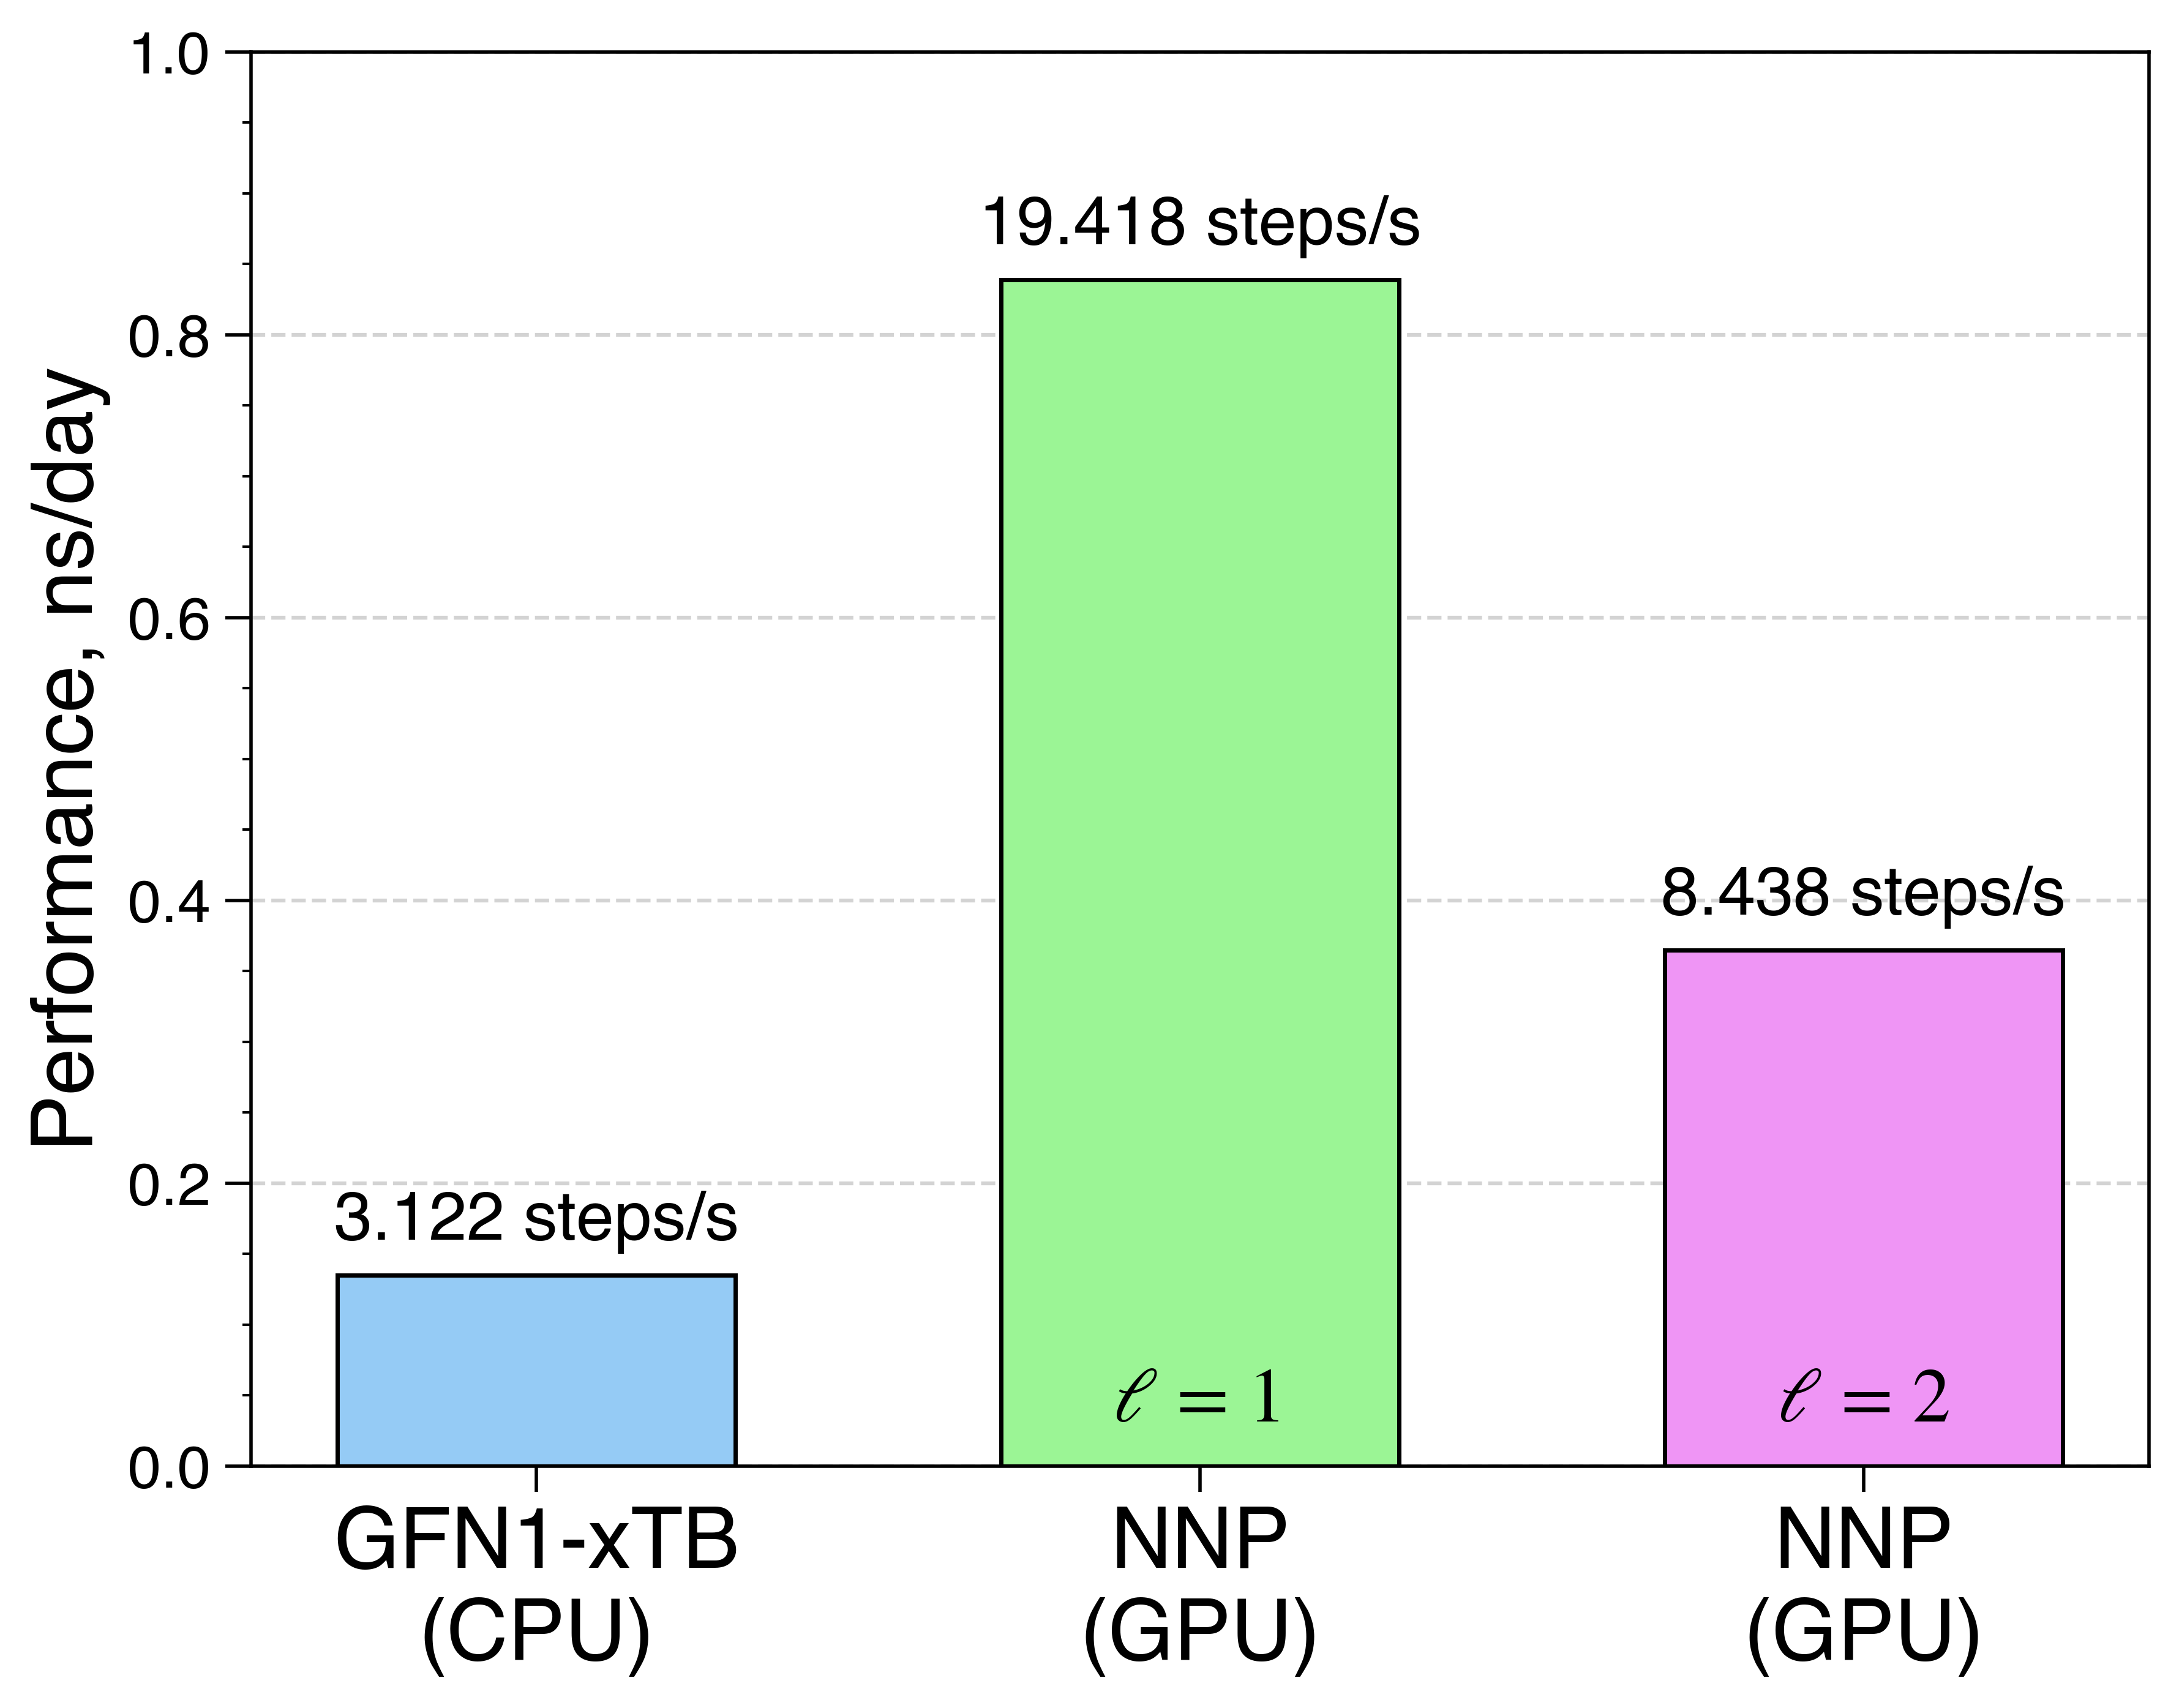
\includegraphics[width=0.6\textwidth]{Figures/4_Results/results_performance_comparison.png}
    \caption{Comparison of the performance between the \textit{ab initio} molecular dynamics runs driven by GFN1-xTB and neural network potentials fitted with the different tensor ranks.}
    \label{fig:performance_comparison}
\end{figure}


%%%%%%%%%%%%%%%%%%%%%%%%%%%%%%%%%%%%%%%%%%%%%%%%%%%%%%%%%%%%%%%%%%%%%%%%%%%%%%%%

\section{Stability of the production runs}



%%%%%%%%%%%%%%%%%%%%%%%%%%%%%%%%%%%%%%%%%%%%%%%%%%%%%%%%%%%%%%%%%%%%%%%%%%%%%%%%

\section{Convergence of the free energy profiles}



%%%%%%%%%%%%%%%%%%%%%%%%%%%%%%%%%%%%%%%%%%%%%%%%%%%%%%%%%%%%%%%%%%%%%%%%%%%%%%%%

\section{Evolution of the collective variables over time}



%%%%%%%%%%%%%%%%%%%%%%%%%%%%%%%%%%%%%%%%%%%%%%%%%%%%%%%%%%%%%%%%%%%%%%%%%%%%%%%%


\section{Reaction mechanism for methyl diphosphate trianion}
\subsection{Minimum free energy path and free energy surface}
\subsection{Proton transfer mechanism}



%%%%%%%%%%%%%%%%%%%%%%%%%%%%%%%%%%%%%%%%%%%%%%%%%%%%%%%%%%%%%%%%%%%%%%%%%%%%%%%%

\section{Reaction mechanism for methyl diphosphate dianion}
\subsection{Minimum free energy path and free energy surface}
\subsection{Proton transfer mechanism}



%%%%%%%%%%%%%%%%%%%%%%%%%%%%%%%%%%%%%%%%%%%%%%%%%%%%%%%%%%%%%%%%%%%%%%%%%%%%%%%%

\section{Arrhenius relationship}



%%%%%%%%%%%%%%%%%%%%%%%%%%%%%%%%%%%%%%%%%%%%%%%%%%%%%%%%%%%%%%%%%%%%%%%%%%%%%%%%

